% Neuroloop utilities - Synthesis model guide - Robinson model - Analysis
% Written by Christopher Thomas.

\section{Model Analysis}
\label{sect-robinson-math}

%
%
\subsection{Low-Pass Filter Delays}
\label{sect-robinson-math-lowpass}

Applying the Laplace transform to Equation \ref{eq-robinson-potential} shows
that the effect of $\alpha$ and $\beta$ is to apply a low-pass filter to the
weighted sum of input firing rates (a second-order exponential smoothing
filter with poles at $-\alpha$ and $-\beta$).

\begin{equation}
\left ( \frac{1}{\alpha \beta} \right ) s^2 V_a(s)
+ \left ( \frac{1}{\alpha} + \frac{1}{\beta} \right ) s V_a(s)
+ V_a(s) = \sum_b \nu_{ab} \Phi_b(s)
\end{equation}
%
\begin{equation}
s^2 V_a(s) + (\alpha + \beta) s V_a(s) + \alpha \beta V_a(s)
= \alpha \beta \sum_b \nu_{ab} \Phi_b(s)
\end{equation}
%
\begin{equation}
(s + \alpha) (s + \beta) V_a(s) = \alpha \beta \sum_b \nu_{ab} \Phi_b(s)
\end{equation}
%
\begin{equation}
\frac{V_a(s)}{\sum_b \nu_{ab} \Phi_b(s)}
= \frac{\alpha \beta}{(s + \alpha) (s + \beta)}
\end{equation}

Applying the Laplace transform to Equation \ref{eq-robinson-gamma} shows
that the effect of $\gamma$ is to apply a low-pass filter to the firing rate
(a second-order exponential smoothing filter with both poles at $-\gamma$).

\begin{equation}
\left ( \frac{1}{\gamma^2} \right ) s^2 \Phi(s)
+ \left ( \frac{2}{\gamma} \right ) s \Phi(s) + \Phi(s) = Q(s)
\end{equation}
%
\begin{equation}
s^2 \Phi(s) + 2 \gamma s \Phi(s) + \gamma^2 \Phi(s) = \gamma^2 Q(s)
\end{equation}
%
\begin{equation}
(s + \gamma)^2 \Phi(s) = \gamma^2 Q(s)
\end{equation}
%
\begin{equation}
\frac{\Phi(s)}{Q(s)} = \frac{\gamma^2}{(s + \gamma)^2}
\end{equation}

The effect of both of these filters is to suppress high-frequency
oscillations (those above the filter corner frequencies) and to delay
low-frequency oscillations by an amount approximately equal to the filters'
time constants. These delays and corner frequencies are listed in Table
\ref{tab-robinson-lowpass} (using the parameter values from
\ref{tab-robinson-params}).

\tabdef{%
\begin{tabular}{cccc}\hline
\textbf{Parameter} & \textbf{Value} & \textbf{Corner} & \textbf{Delay} \\
\hline
$\alpha$ & 50 sec$^{-1}$ & 8 Hz & 20 ms \\
$\beta$ & 200 sec$^{-1}$ & 32 Hz & 5 ms \\
$\gamma$ & 100 sec$^{-1}$ & 16 Hz & 20 ms$^*$ \\
\hline
\multicolumn{4}{l}
{\footnotesize $^*$Each pole at $-\gamma$ introduces a 10~ms delay; there
are two such poles.}
\end{tabular}
}{Robinson model low-pass filter corners and low-frequency delays.}
{tab-robinson-lowpass}

%
%
\subsection{Oscillation Modes and Oscillation Criteria}
\label{sect-robinson-math-modes}

A simplified diagram of the extended Robinson model is shown in Figure
\ref{fig-robinson-loops}. This is intended to make it easy to identify the
feedback loops that may support oscillations. Blue arcs indicate positive
coefficients, and red arcs indicate negative (inhibitory) coefficients.
As an approximation, the activity of different excitatory neuron populations
within the cortex is assumed to be the same, combining $\nu_{ee}$ and
$\nu_{ee\_ext}$. Additionally, multiplicative portion of the noise is
treated as a contribution to the $\nu_{se}$ arc. The average contribution of
the $\chi \sigma_n \nu_n$ term is zero, but the magnitude of that term
compared to the magnitude of $\nu_{se}$ indicates whether or not
multiplicative noise significantly contributes to that arc.

\figdef{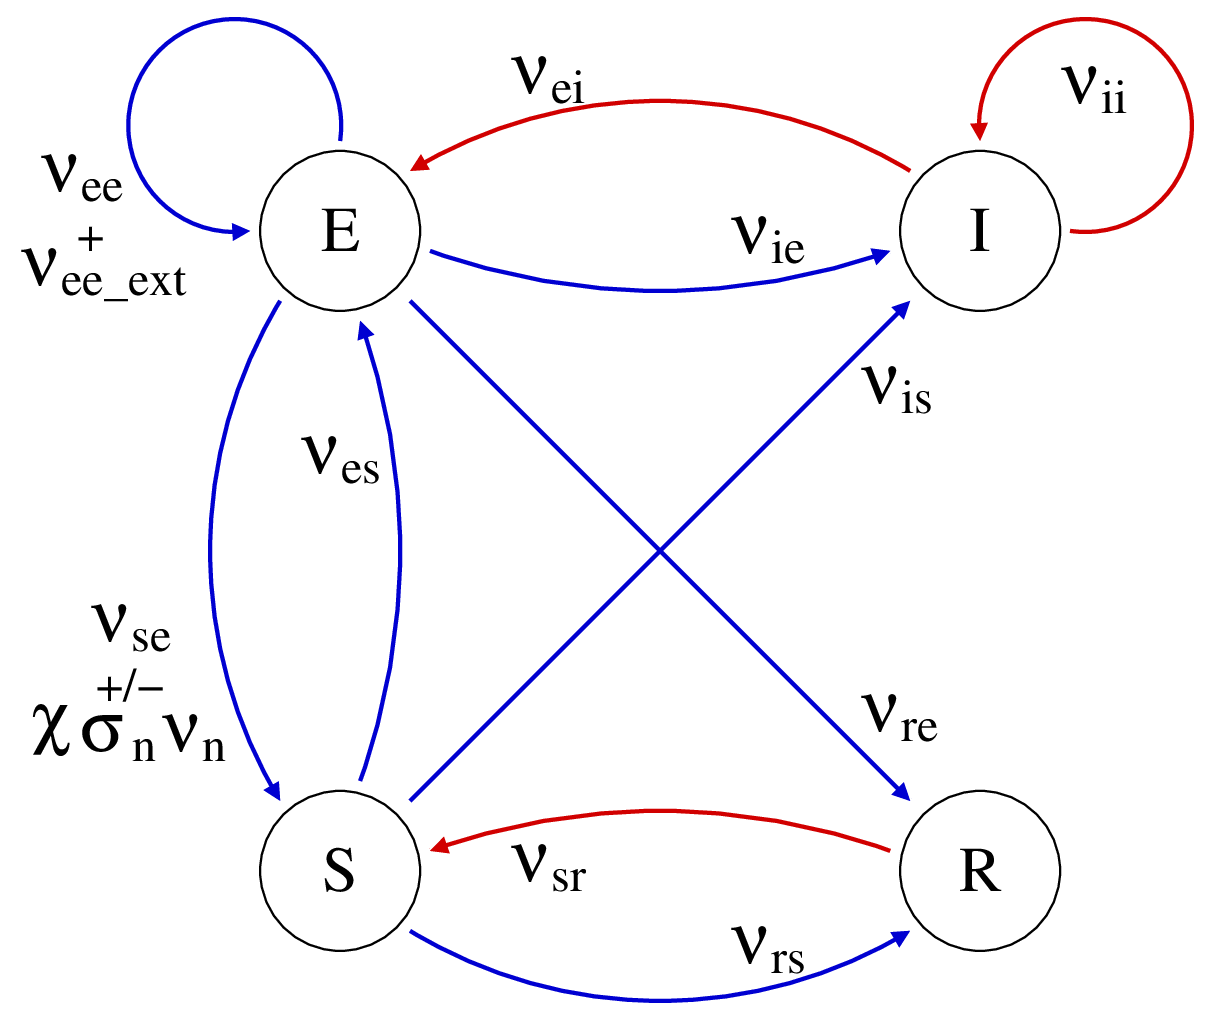
\includegraphics[height=2.5in]{figures/robinson-model-loops}}
{Simplified diagram of the extended Robinson model, showing feedback loops.}
{fig-robinson-loops}

A list of potential oscillation loops and their oscillation frequencies is
given in Table \ref{tab-robinson-loops}. For loops consisting entirely of
positive coefficients, the oscillation period is the time needed to complete
a single circuit. For loops with one negative coefficient, the oscillation
period is the time needed to complete two circuits around the loop (in the
same manner as a ring oscillator). Harmonics of these oscillation frequencies
are also supported.

The number of arc traversals needed for one oscillation period is noted.
Per above, this may reflect either one or two cycles around the loop. Each
arc traversal involves gain from arc coefficients (noted in the table),
small-signal gain from the $Q(V)$ transfer function (omitted from the table),
and delay from the $\alpha$ and $\beta$ filter components. Delay
contributions from the cortex excitatory population $\gamma$ filter
component and from the cortex-thalamus loop are noted in the table where
applicable.

\tabdef{%
\begin{tabular}{ccccccc}\hline
\textbf{Label} & \textbf{Arcs} & \textbf{Gamma} & \textbf{C-T Loop} &
\textbf{Period} & \textbf{Frequency} & \textbf{Gain} \\
\hline
ES & 2 & Y & Y & 150 ms & 6.7 Hz & $\nu_{se} \cdot \nu_{es}$ \\
EE & 1 & Y & -- & 45 ms & 22 Hz & $\nu_{ee} + \nu_{ee\_ext}$ \\
\hline
EI & 4 & Y & -- & 140 ms & 7 Hz & $2 \cdot \nu_{ie} \cdot \nu_{ei}$ \\
SR & 4 & -- & -- & 100 ms & 10 Hz & $2 \cdot \nu_{rs} \cdot \nu_{sr}$ \\
%
ERS & 6 & Y & Y & 350 ms & 2.9 Hz &
$2 \cdot \nu_{re} \cdot \nu_{sr} \cdot \nu_{es}$ \\
ESI & 6 & Y & Y & 350 ms & 2.9 Hz &
$2 \cdot \nu_{se} \cdot \nu_{is} \cdot \nu_{ei}$ \\
\hline
\end{tabular}
}{Extended robinson model oscillation modes. Top two modes: single-cycle.
Bottom four modes: two-cycle (inverting).}
{tab-robinson-loops}

Resonant loops explicitly described in Section IV of Robinson 2002 are the
ones marked ES, ERS, and SR. The oscillation periods described in Section
V of Robinson 2002 are consistent with the estimated periods of the ERS and
SR loops in Table \ref{tab-robinson-loops}.

The authors of Robinson 2002 were primarily concerned with noise-excited
oscillations, and so only evaluated oscillation loops that included the
specific nucleus. Evaluation was expressed in terms of the transfer
function from the noise signal (input) to the firing rate of cortex
excitatory neurons (output). Resonant oscillations were presumed to occur
at frequencies for which this transfer function diverged (producing
arbitrarily large output for finite input). This work instead considers
gain within a loop, with resonant oscillations corresponding to a loop
gain exceeding unity. As this does not explicitly consider noise excitation,
all of the loops described in Table \ref{tab-robinson-loops} may be
analyzed.

\subsection{Operating Points and Parameter Choices}
\label{sect-robinson-math-fixed}

As was described in Robinson 2002, the dynamics of the extended Robinson
model can be analyzed by considering unchanging (DC) firing rates, and
evaluating the small-signal gain around these operating points. While this
was used to find the transfer function
$\frac{\phi_e(\omega)}{\phi_n(\omega)}$ in Robinson 2002, here it is used
to find the small-signal loop gain (to determine which oscillating modes
are dominant for given parameter values).

At a given operating point, the sensitivity of the gain of the dominant
loops to each of the $v_{ab}$ coefficients provides insight into which
network connections are most relevant for influencing dynamcis at that
operating point. $v_{ee\_ext}$ is particularly of interest, as this
may be used as a proxy for the sensitivity of network dynamics to changes
in the connectivity matrix between different excitatory cortex neuron
populations.

For time-independent operating point analysis, Equation
\ref{eq-robinson-potential} reduces to:

\begin{equation}
V_a(t) = \sum_b \nu_{ab} \phi_b(t)
\label{eq-robinson-dc-potential}
\end{equation}

Equation \ref{eq-robinson-sigmoid} is unchanged, and Equation
\ref{eq-robinson-gamma} reduces to:

\begin{equation}
\phi_a(t) = Q(V_a(t))
\label{eq-robinson-dc-nogamma}
\end{equation}

The gain $G_{ab}$ of any given arc is the derivative of its output firing
rate with respect to its input firing rate. For oscillations with
frequencies much lower than the $\alpha$, $\beta$, and $\gamma$ filter
corner frequencies, this may be estimated by taking the derivative of the
DC operating point equations (rather than requiring an analysis of the full
system dynamics):

\begin{equation}
G_{ab} = \frac{d\phi_a}{d\phi_b} = \frac{d}{d\phi_b} \left [ Q(V_a) \right ]
\end{equation}

\begin{equation}
G_{ab} = Q'(V_a) \frac{dV_a}{d\phi_b}
\end{equation}

\begin{equation}
G_{ab} = Q'(V_a) \frac{d}{d\phi_b} \left [ \sum_c \nu_{ac} \phi_c \right ]
\end{equation}

\begin{equation}
G_{ab} = Q'(V_a) \nu_{ab}
\label{eq-robinson-gain-qprime}
\end{equation}

The sigmoid response function is defined in terms of the logistic function:

\begin{equation}
\left \{
\begin{array}{l}
Q(V) = Q_{max} L \left (\frac{V - V_{th}}{\sigma'_{th}} \right ) \\
\\
L(x) = \frac{1}{1 + e^{-x}} = \frac{e^x}{1 + e^x} \\
\\
\sigma'_{th} = \frac{\sqrt{3}}{\pi}\sigma_{th} \\
\end{array}
\right .
\label{eq-robinson-sigmoid-logistic}
\end{equation}

The derivative of the logistic function is:

\begin{equation}
L'(x) = L(x) \left ( 1 - L(x) \right ) = \frac{e^x}{(1 + e^x)^2}
\label{eq-robinson-logistic-derivative}
\end{equation}

This gives the derivative of the sigmoid response function:

\begin{equation}
Q'(V) = Q_{max} L' \left ( \frac{V - V_{th}}{\sigma'_{th}} \right )
\frac{d}{dV} \left [ \frac{V - V_{th}}{\sigma'_{th}} \right ]
\end{equation}

\begin{equation}
Q'(V) = \frac{Q_{max}}{\sigma'_{th}}
L' \left ( \frac{V - V_{th}}{\sigma'_{th}} \right )
\end{equation}

\begin{equation}
Q'(V) = \frac{Q_{max}}{\sigma'_{th}}
L \left ( \frac{V - V_{th}}{\sigma'_{th}} \right )
\left ( 1 - L \left ( \frac{V - V_{th}}{\sigma'_{th}} \right ) \right )
\end{equation}

\begin{equation}
Q'(V) = \frac{Q_{max}}{\sigma'_{th}}
L \left ( \frac{V - V_{th}}{\sigma'_{th}} \right )
\left ( 1 - \frac{Q_{max}}{Q_{max}}
L \left ( \frac{V - V_{th}}{\sigma'_{th}} \right ) \right )
\end{equation}

\begin{equation}
Q'(V) = \frac{1}{\sigma'_{th}} Q(V) \left ( 1 - \frac{Q(V)}{Q_{max}} \right )
\end{equation}

Combining this with Equation \ref{eq-robinson-gain-qprime} gives:

\begin{equation}
G_{ab} = \frac{\nu_{ab}}{\sigma'_{th}}
Q(V_a) \left ( 1 - \frac{Q(V_a)}{Q_{max}} \right )
\end{equation}

\begin{equation}
G_{ab} = \frac{\nu_{ab}}{\sigma'_{th}}
\phi_a \left ( 1 - \frac{\phi_a}{Q_{max}} \right )
\label{eq-robinson-gain}
\end{equation}

This is Equation 10 from Robinson 2002. The small-signal gain of a loop at
low frequencies is the product of $G_{ab}$ for each arc in the loop
(as with the $S_d$, $S_i$, and $S_r$ values in section IV of Robinson 2002).

\fixme{Show how to find operating points. Pick regions of parameter space
from Robinson and also note where Hindriks' parameters were in that space.
Evaluate loop gains at these locations and their sensitivity to weights.
Add an area sensitive to mixing matrix weights if we don't already have one.}

%
%
% This is the end of the file.
